% !TEX root = main.tex

%%%%%%%%%%%%%%%%%%%%%%%%%%%%%%%%%%%%%%%%%%%%%%%%%%%%%%%%%%%%%%%%%%%%%%%%%%%%%%%%%%%%%%%%%%%%%%%%
\section{演習課題}
%%%%%%%%%%%%%%%%%%%%%%%%%%%%%%%%%%%%%%%%%%%%%%%%%%%%%%%%%%%%%%%%%%%%%%%%%%%%%%%%%%%%%%%%%%%%%%%%

\subsection{$f=f_L,f_H$の場合}
\begin{figure}[H]
    \begin{center}
        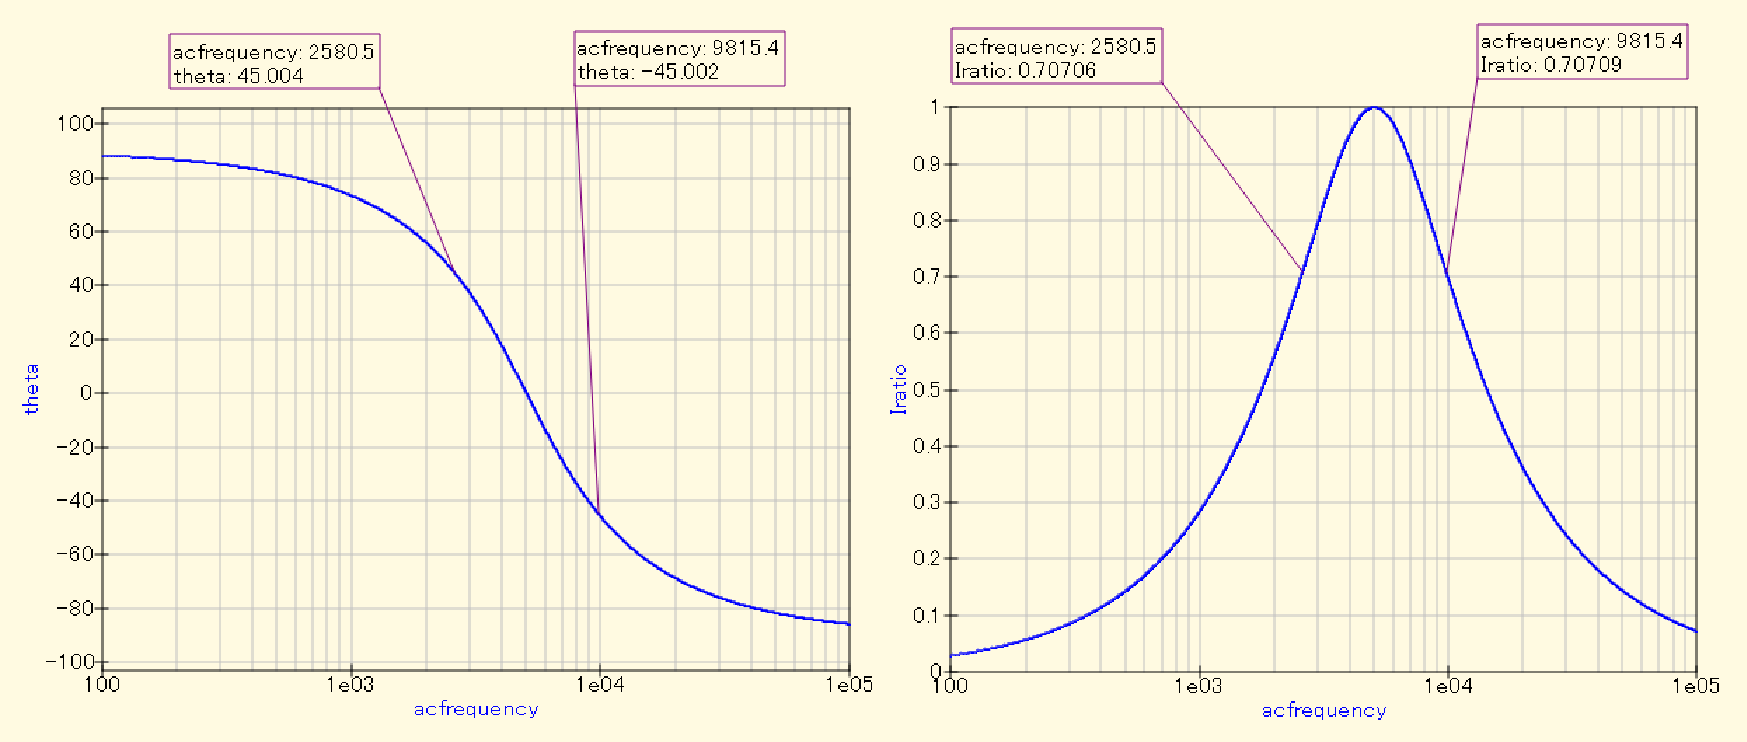
\includegraphics[scale=0.5]{45.pdf}
        \caption{理想コイルにおける$f=f_L,f_H$の場合のインピーダンス偏角の周波数特性}
    \end{center}
\end{figure}

$f=f_L,f_H$においてインピーダンス偏角はそれぞれarg\,$Z=45^\circ,-45^\circ$となる.

\subsection{理想コイルとそうでない場合の比較}
\begin{figure}[H]
    \begin{center}
        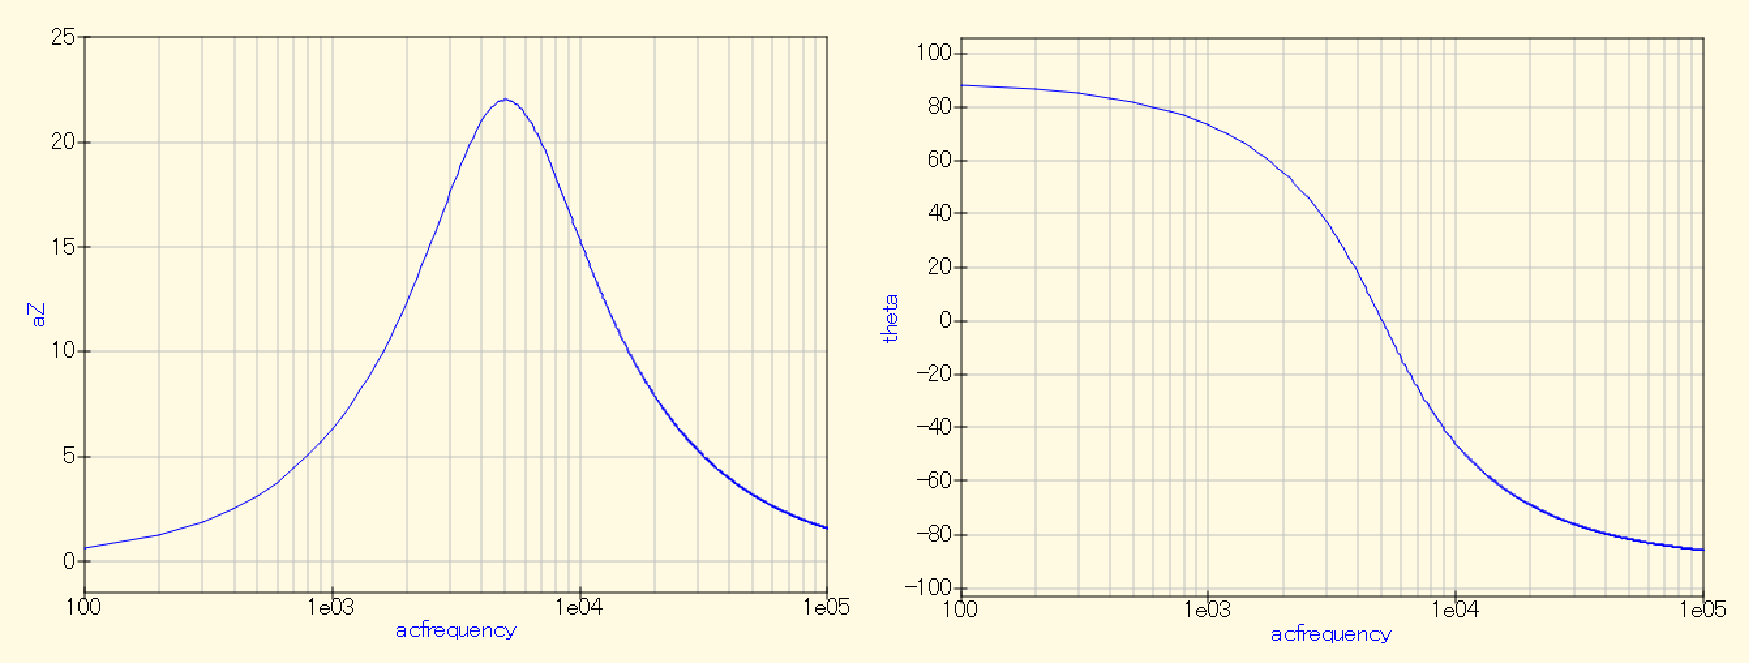
\includegraphics[scale=0.5]{ideal.pdf}
        \caption{理想コイルにおけるインピーダンス周波数特性およびインピーダンス偏角の周波数特性}
    \end{center}
\end{figure}

\begin{figure}[H]
    \begin{center}
        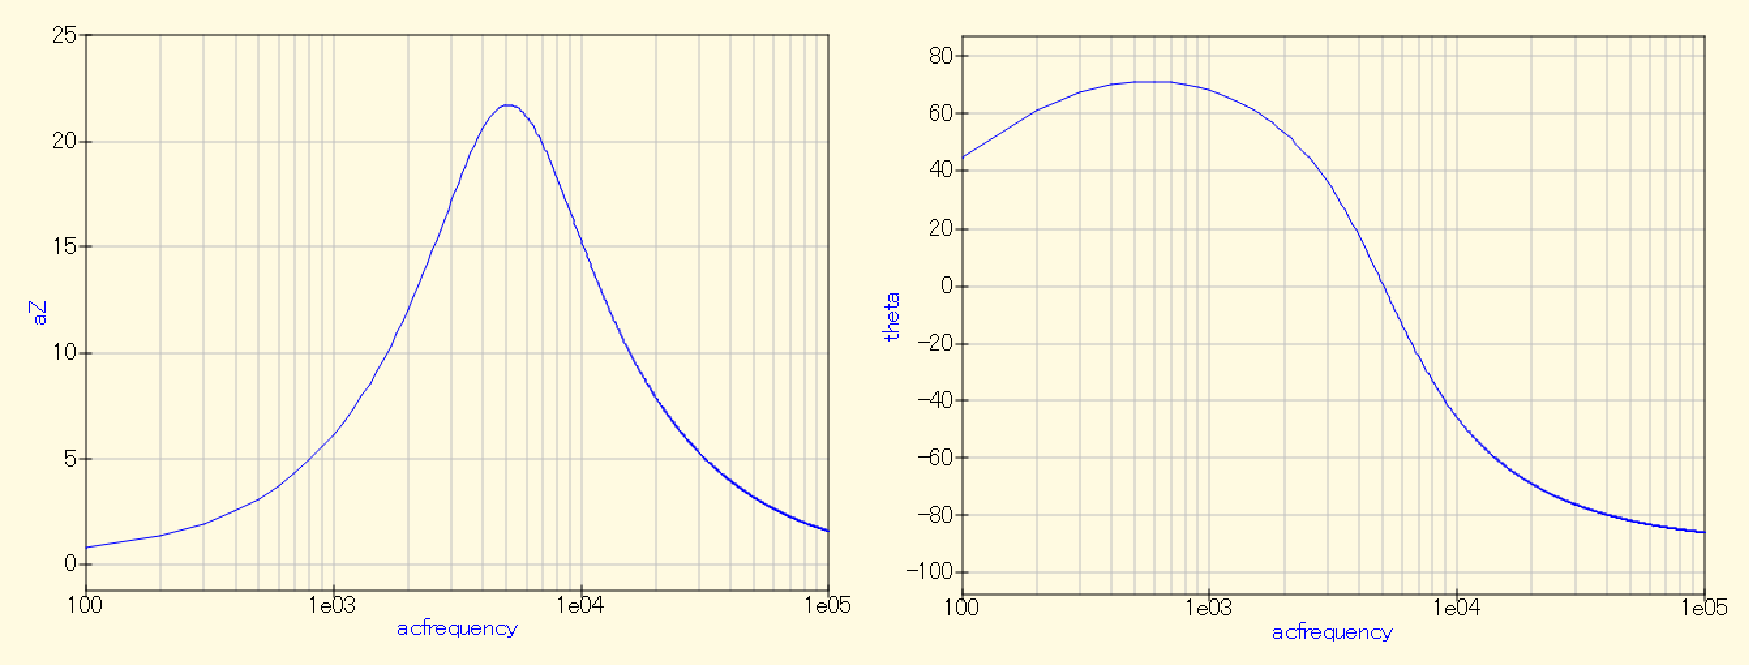
\includegraphics[scale=0.5]{not_ideal.pdf}
        \caption{理想でないコイルにおけるインピーダンス周波数特性およびインピーダンス偏角の周波数特性}
    \end{center}
\end{figure}

インピーダンスの大きさの周波数特性では顕著な差は見られないが,
インピーダンスの偏角の周波数特性では顕著な差が見られる.